\documentclass[twocolumn,a4j]{jsarticle}
\setlength{\topmargin}{-20.4cm}
\setlength{\oddsidemargin}{-10.4mm}
\setlength{\evensidemargin}{-10.4mm}
\setlength{\textwidth}{18cm}
\setlength{\textheight}{26cm}

\usepackage[top=15truemm,bottom=25truemm,left=15truemm,right=15truemm]{geometry}
\usepackage[latin1]{inputenc}
\usepackage{amsmath}
\usepackage{amsfonts}
\usepackage{amssymb}
\usepackage[dvipdfmx]{graphicx}
\usepackage[dvipdfmx]{color}
\usepackage{listings}
\usepackage{listings,jvlisting}
\usepackage{geometry}
\usepackage{framed}
\usepackage{color}
\usepackage[dvipdfmx]{hyperref}
\usepackage{ascmac}
\usepackage{enumerate}
\usepackage{tabularx}
\usepackage{cancel}
\usepackage{scalefnt}

\renewcommand{\figurename}{Fig.}
\renewcommand{\tablename}{Table }

\lstset{
basicstyle={\ttfamily},
identifierstyle={\small},
commentstyle={\smallitshape},
keywordstyle={\small\bfseries},
ndkeywordstyle={\small},
stringstyle={\small\ttfamily},
frame={tb},
breaklines=true,
columns=[l]{fullflexible},
xrightmargin=0zw,
xleftmargin=3zw,
numberstyle={\scriptsize},
stepnumber=1,
numbersep=1zw,
lineskip=-0.5ex
}

\makeatletter
\def\@maketitle
{
\begin{center}
{\LARGE \@title \par}
\end{center}
\begin{flushright}
{\large 報告書 NO.06 - 1\quad\@date\quad\@author}
\end{flushright}
\par\vskip 1.5em
}
\makeatother

\setcounter{tocdepth}{3}

\author{来代 勝胤}
\title{令和3年度 10月 第2週 報告書}
\date{2021/10/14}

\begin{document}
\columnseprule=0.1mm

\maketitle
\section*{報告内容}
\begin{enumerate}[1.]
    \item 進捗状況
    \item ロードセルと荷重の関係式の導出
    \item ロードセルとひずみセンサの関係式の導出
    \item 
\end{enumerate}
\section{進捗状況}
今週は、校正実験データから、以下の手順で\\
ひずみセンサからの出力を実際の入力へと換算を行った。
\begin{enumerate}[(1)]
    \item ロードセルと荷重の関係式の導出
    \item 
\end{enumerate}
\section{ロードセルと荷重の関係式の導出}
2021年6月18日に実施した実験結果より、
ロードセルと荷重の関係式を算出した。\par
ロードセルの出力(横軸)及びロードセルの引張方向に入力した荷重(縦軸)の関係を
表した図は、以下の Fig.1 のようになった。
\begin{figure}[htbp]
    \footnotesize
    \begin{center}
        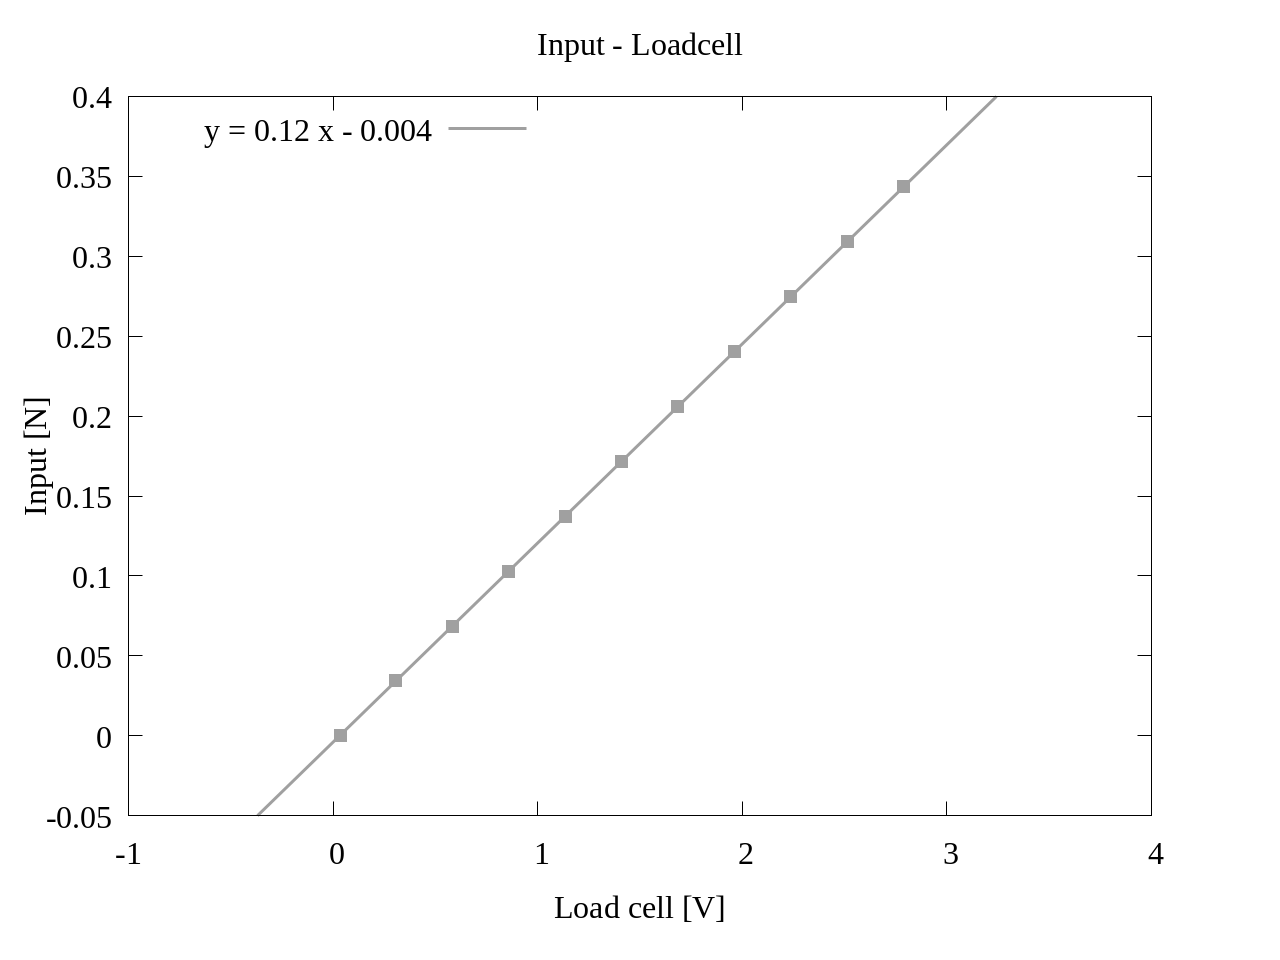
\includegraphics[width=90mm]{images/02_force&line.png}
        \caption{Loadcell's input and output}
    \end{center}
\end{figure}

また、近似直線は、$x$をロードセルの出力、$y$を荷重として、
以下の式(1)の結果を得ることができた。
\begin{eqnarray}
    y = 0.12 x - 0.004
\end{eqnarray}

\newpage

\section{ロードセルとひずみセンサの関係式の導出}
2021年6月21日に実施した実験結果より、
ロードセルとひずみセンサの関係式を導出した。\\

\subsection{各センサとロードセルの押込み距離の関係}
実験の操作により、ロードセルをタイヤモデルに接触させ、
x軸(抗力)方向及びy軸(揚力)方向に任意の距離だけ押込み
それぞれロードセル及びタイヤモデルに取り付けられた
2つのひずみセンサのセンサについて測定した。\par
以下の Fig.2 及び Fig.3 はx軸(抗力)方向及びy軸(揚力)方向について、
ロードセルの押込み距離(横軸)と各センサの出力の関係(縦軸)を示している。
\begin{figure}[htbp]
    \footnotesize
    \begin{center}
        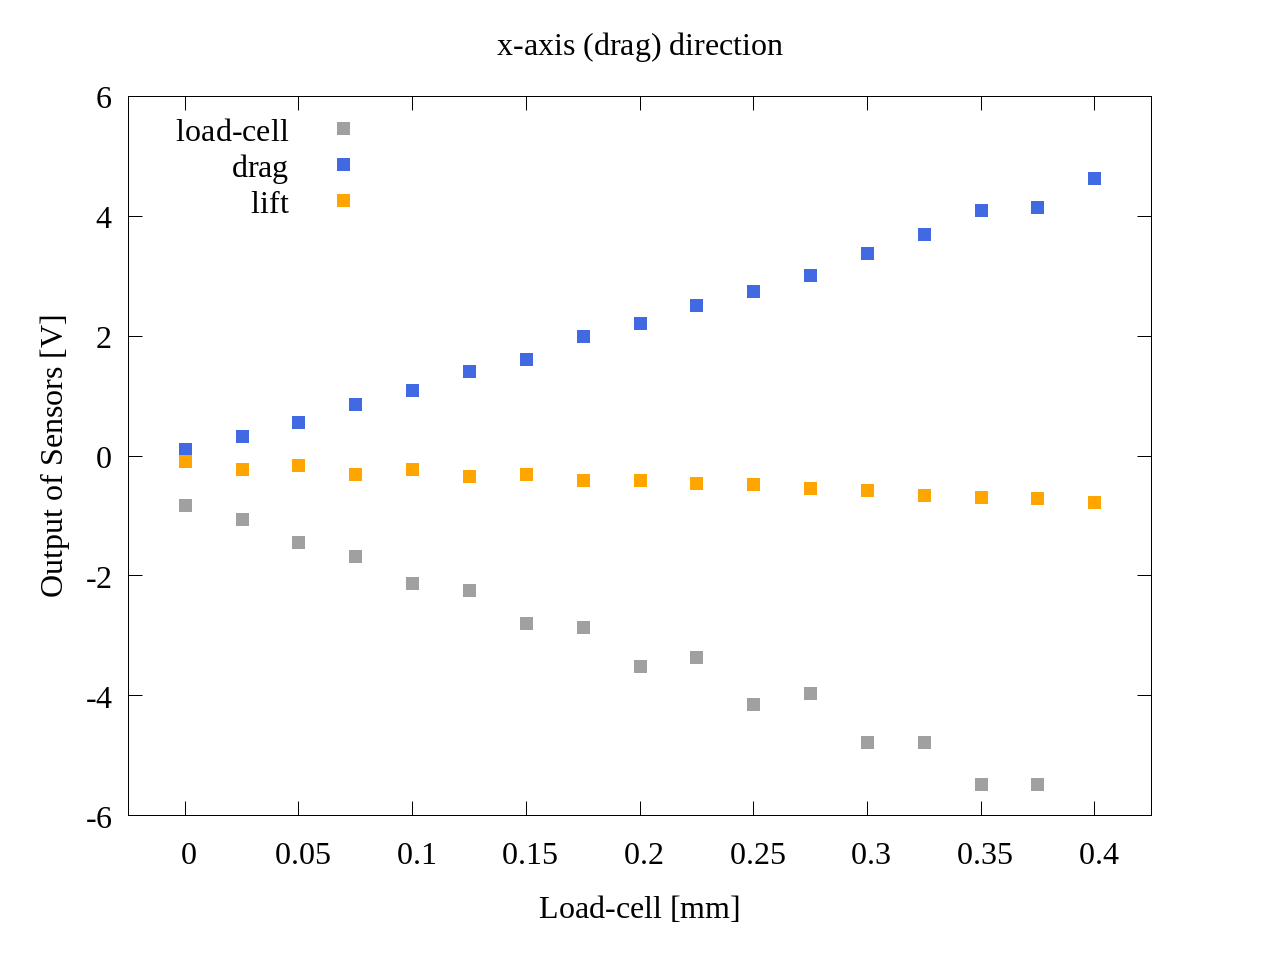
\includegraphics[width=90mm]{images/03_length-output_x.png}
        \caption{Correlation between length and output (x-axis)}
        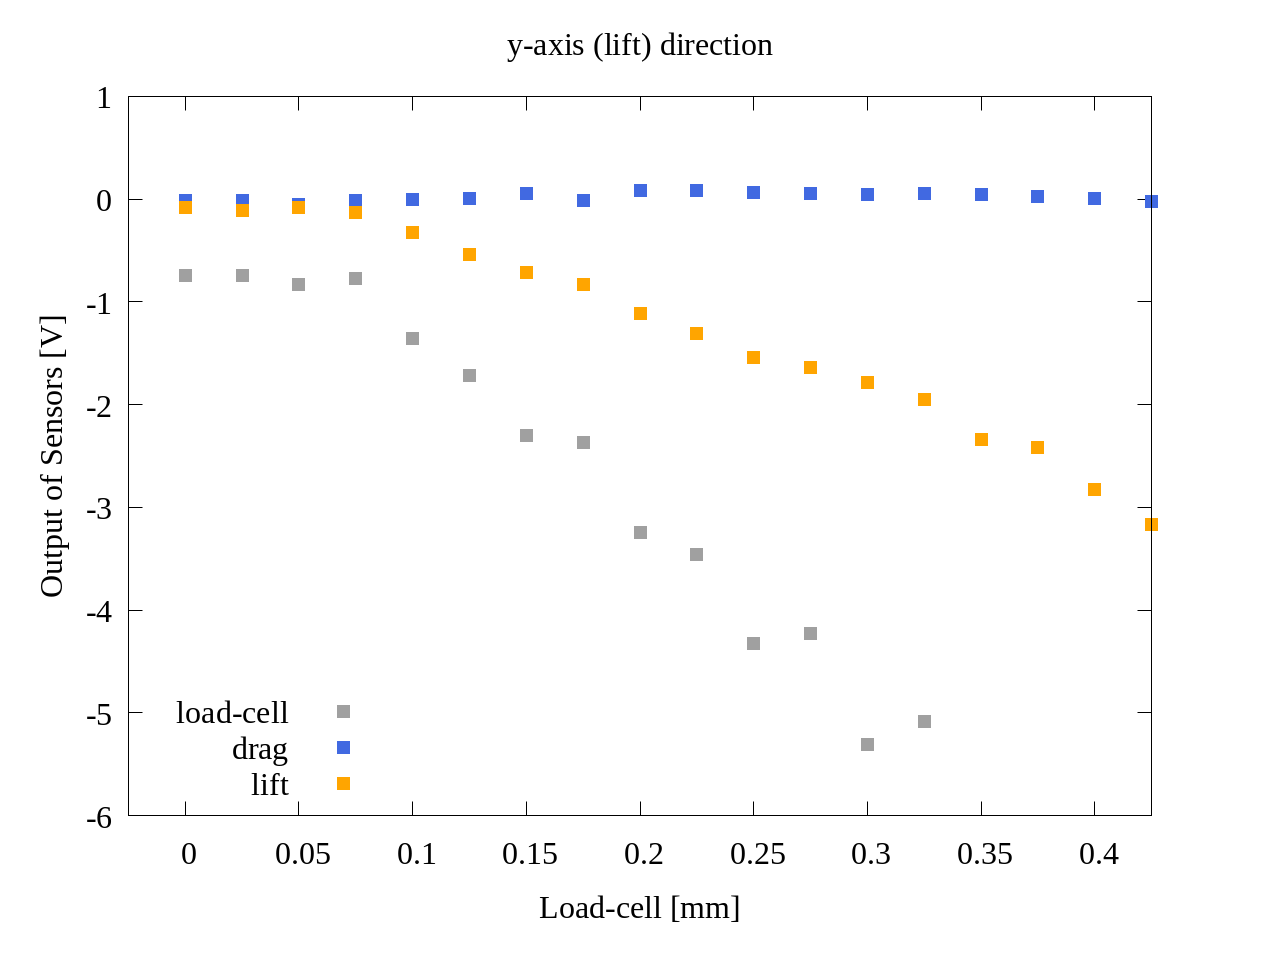
\includegraphics[width=90mm]{images/04_length-output_y.png}
        \caption{Correlation between length and output (y-axis)}
    \end{center}
\end{figure}

\subsection{ロードセルとひずみセンサの出力の関係}
ロードセルの出力(横軸)とタイヤモデルに取り付けられた
ひずみセンサの出力(縦軸)の関係を以下のFig. 4、Fig.5に示す。
\begin{figure}[htbp]
    \footnotesize
    \begin{center}
        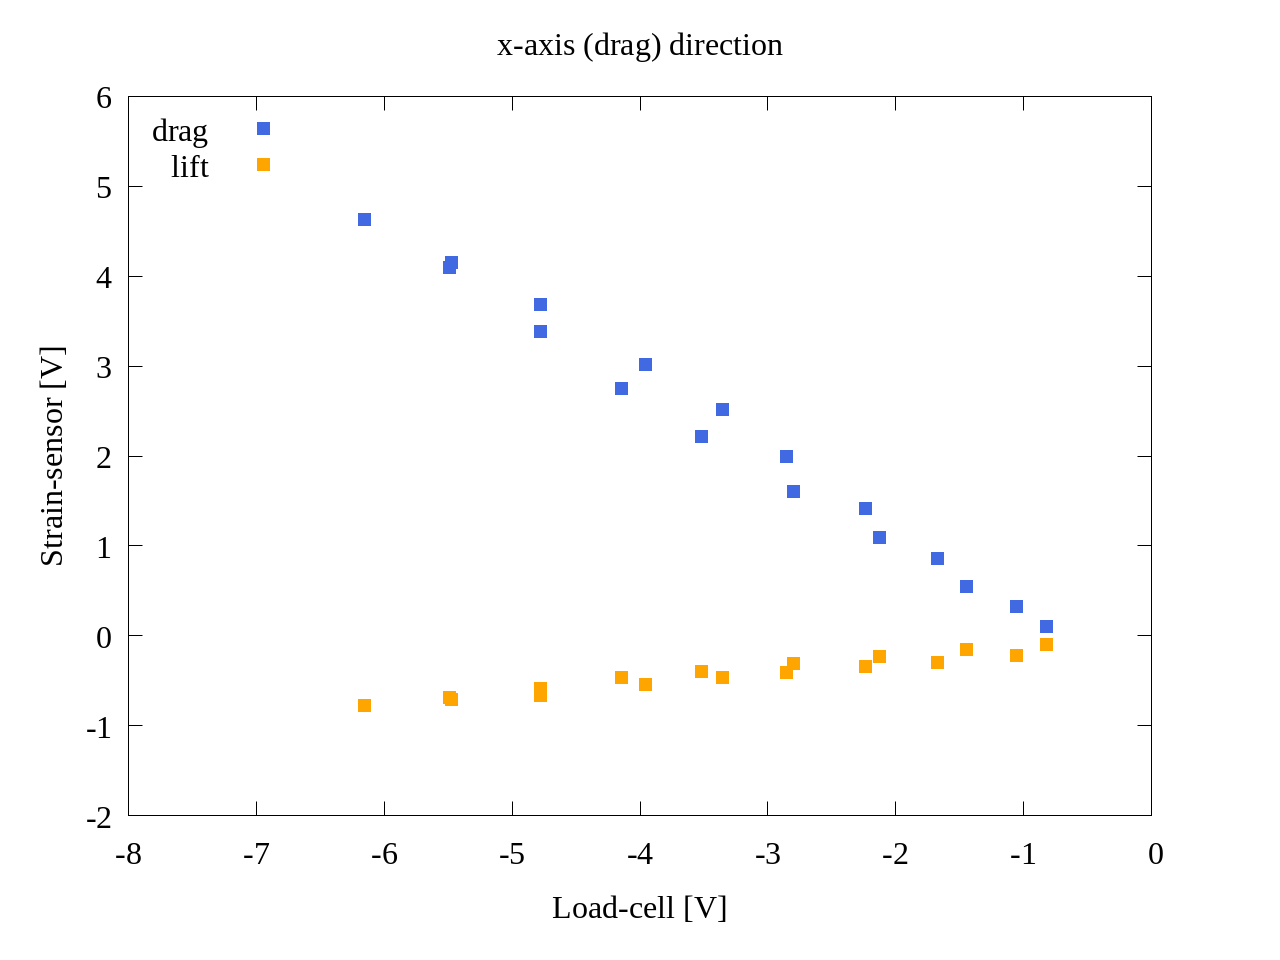
\includegraphics[width=90mm]{images/05_strainsensor-loadcell_x.png}
        \caption{Correlation of load-cell and strain-sensors (x-axis)}
        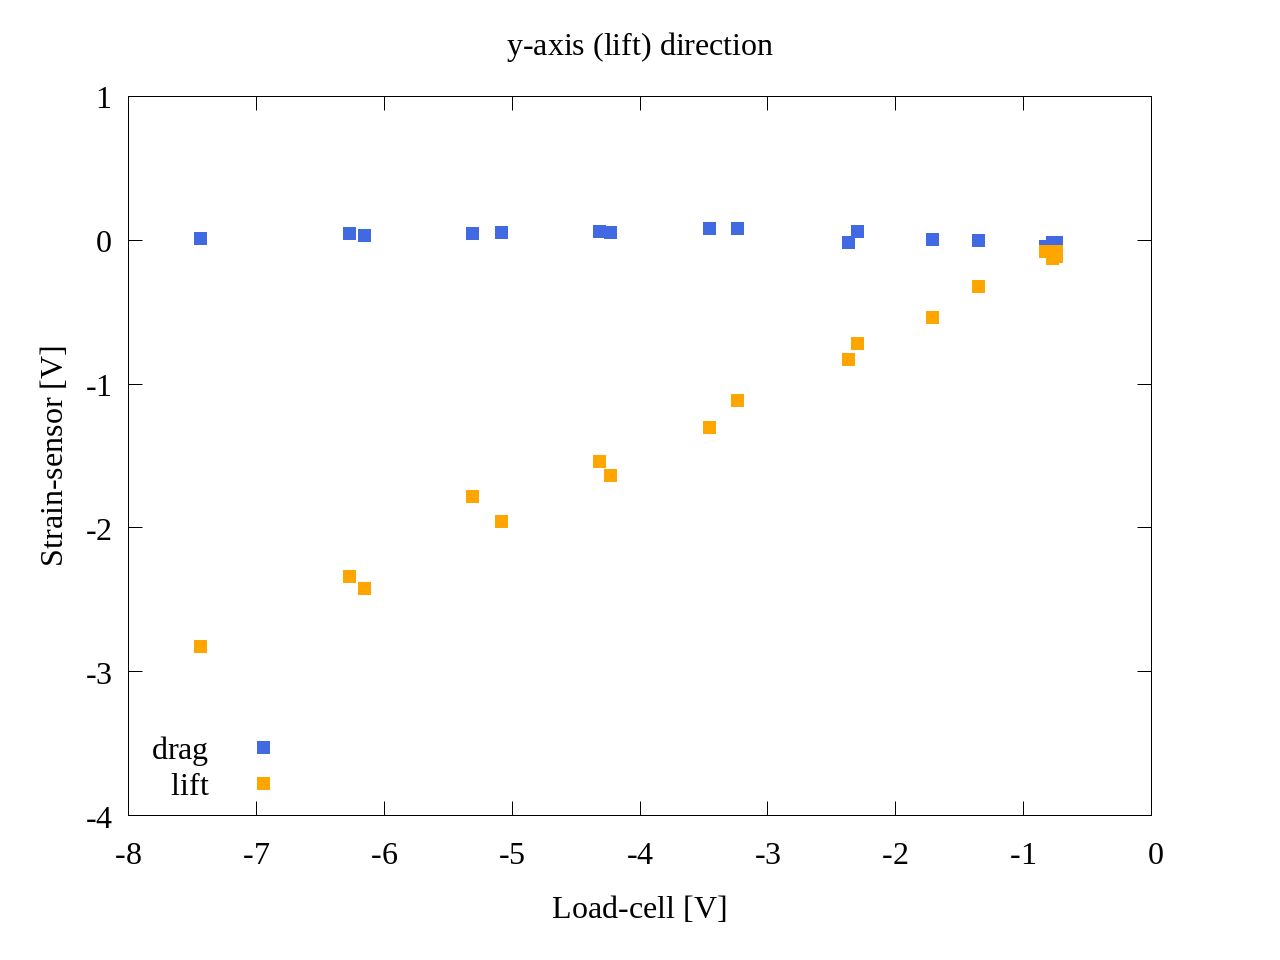
\includegraphics[width=90mm]{images/06_strainsensor-loadcell_y.png}
        \caption{Correlation of load-cell and strain-sensors (y-axis)}
    \end{center}
\end{figure}

\newpage
\section{ひずみセンサと入力荷重の関係式の算出}
Fig.1,Fig.4 の "drag" 、Fig.5の "lift" の結果から、ひずみセンサの出力(横軸)と入力荷重(縦軸)の関係について
以下の Fig.6 に示す。
\begin{figure}[htbp]
    \footnotesize
    \begin{center}
        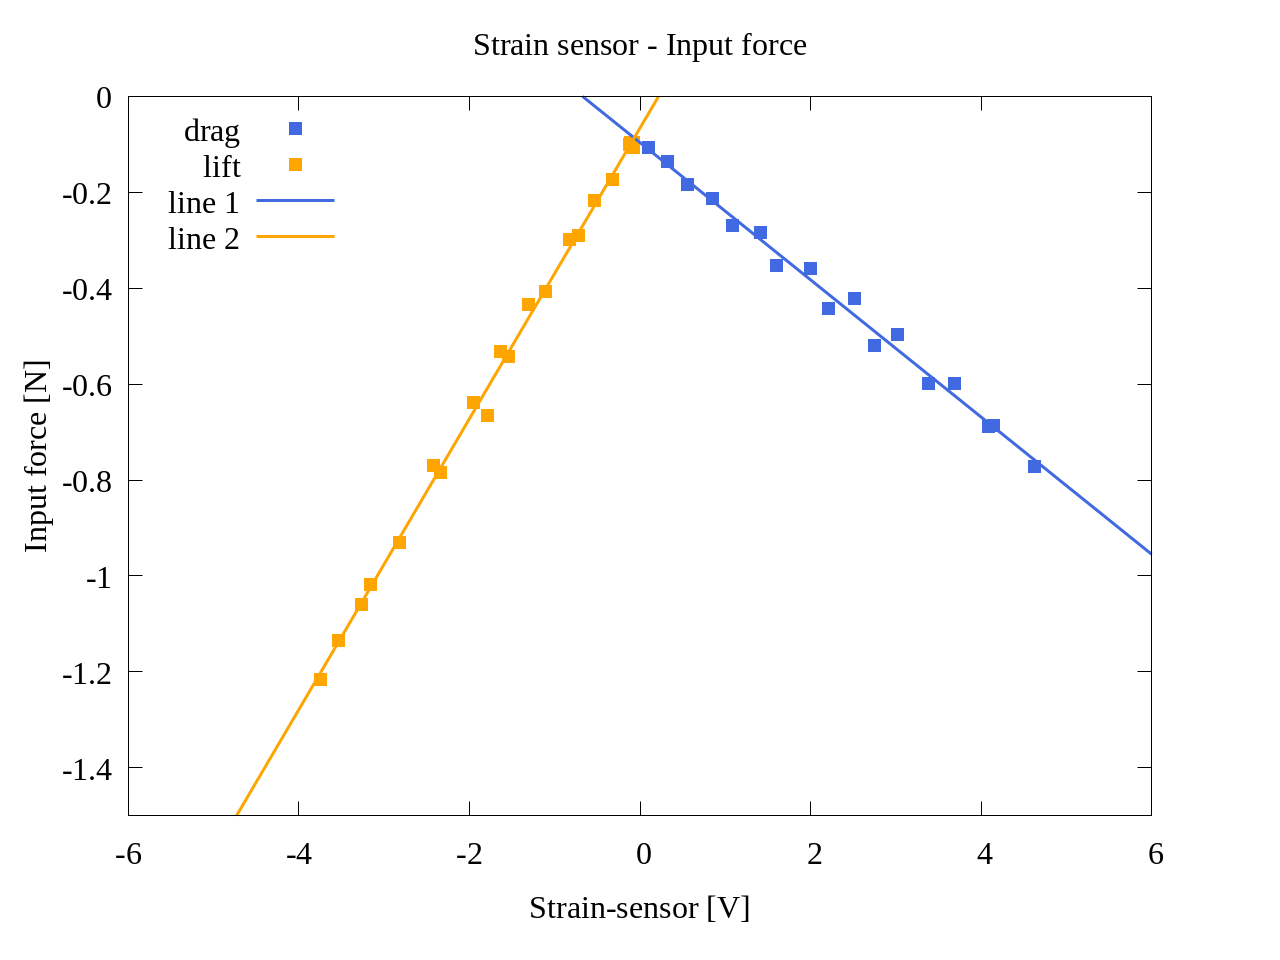
\includegraphics[width=90mm]{images/08_strainsensor-forces&line.png}
        \caption{}
    \end{center}
\end{figure}

また、drag 及び lift に対して、それぞれ以下の式(2)、式(3)の近似直線を得た。
\begin{eqnarray}
    \mathrm{line 1} \; : \; y &=& -0.143 \; x - 0.10\\
    \mathrm{line 2} \; : \; y &=& 0.303 \; x - 0.07
\end{eqnarray}

\section{実験データの荷重への換算}



\section{今後の予定}
\end{document}